% !TEX root = ../thesis.tex

\chapter{Analytická časť}

Analytická časť záverečnej práce analyzuje existujúce podobné prístupy k~riešeniu stanoveného problému. Autor práce musí uviesť v~tejto časti existujúce prístupy a riešenia, pričom musí zaujať stanovisko k~týmto prístupom a riešeniam a opísať ich výhody a nedostatky. Prevažne v~tejto časti autor používa odkazy na použité zdroje. Autor v~analýze nepreberá odseky z~cudzích prác ale uvádza prevažne vlastné postoje podložené odkazmi na literatúru. Analytická časť práce by teda nemala byť len povrchným prepisom základných informácií z~Wikipédie alebo zo stránok opisovaných nástrojov. Je potrebné aby bola analýza podporená aj experimentmi ak to umožňuje téma práce (napr. vyskúšam softvér). Vďaka popisu existujúcich riešení autor pochopí problematiku, viac sa nad riešeniami zamyslí, usporiada si ich, zistí ich kladné a záporné vlastnosti, z~čoho potom postupne vyplynie návrh vlastného riešenia v~syntetickej časti. Analytická časť tvorí zvyčajne ¼ jadra práce.

Analytickú časť je možné rozdeliť na niekoľko kapitol, ktoré budú venované rôznym analyzovaným témam. Názvy kapitol majú zodpovedať tomu, čo je v~kapitole opisované. Napríklad ak v~práci analyzujete súčasný stav v~oblasti medzigalaktických letov, namiesto všeobecného názvu "`Analýza súčasného stavu"' by mal byť použiťý názov analyzovanej témy --- "`Medzigalaktické lety"'.

% lorem ipsum
\section{Lorem ipsum}
\blindtext

\section{Aliquam eu malesuada urna}
\blindtext
\begin{itemize}
    \item v~knihe \cite{book} autor prezentuje naozaj odvážne myšlienky
    \item nemenej zaujímavé výsledky publikuje ďalší autor v~článku \cite{article} 
    \item v~konferenčnom príspevku \cite{conference} sú uvedené tiež zaujímavé veci
    \item \LaTeX{}\footnote{\url{https://www.latex-project.org/}} je typografický jazyk
\end{itemize}

Given a set of numbers, there are elementary methods to compute its \acrlong{gcd}, which is abbreviated \acrshort{gcd}. This process is similar to that used for the \acrfull{lcm}.

\subsection{Donec vehicula consequat}
\blindtext

\begin{figure}[!ht]
    \centering
    
\includegraphics[width=.9\textwidth]{figures/tugboat}
    \caption{\LaTeX{} Friendly Zone \label{o:latex_friendly_zone}}
\end{figure}

\subsection{Nullam in mauris consectetur}
\blindtext

\begin{lstlisting}[language=C,caption={Program, ktorý pozdraví celý svet}]
#include <stdio.h>
int main() {
    /* Print Hello, World! */
    printf("Hello, World!\n");
    return 0;
}
\end{lstlisting}


\subsection{Vestibulum tristique elementum varius}
\blindtext

\begin{table}[!ht]
	\caption{Country list}\label{t:1}
	\smallskip
	\centering

	\begin{tabular}{ |p{3cm}||p{3cm}|p{3cm}|p{3cm}|  }
		\hline
		\multicolumn{4}{|c|}{Country List} \\
		\hline
		Country Name or Area Name& ISO ALPHA 2 Code &ISO ALPHA 3 Code&ISO numeric Code\\
		\hline
		Afghanistan & AF & AFG & 004\\
		Aland Islands & AX & ALA & 248\\
		Albania & AL & ALB & 008\\
		Algeria & DZ & DZA & 012\\
		American Samoa & AS & ASM & 016\\
		Andorra & AD & AND & 020\\
		Angola & AO & AGO & 024\\
		\hline
	\end{tabular}
\end{table}


\section{Phasellus id pretium neque}
\blindtext

\blindtext

\chapter{Analýza}
\section{Analýza všeobecného Web Crawlera}

Web Crawler, tiež nazývaný ako Spider, je webový bot, ktorý na základe jedného alebo viacerých východiskových URL adries stiahne webové stránky s nimi spojené. Extrahuje hyperlinky obsiahnuté na týchto stránkach a následne pokračuje rekurzívne v sťahovaní webových stránok identifikovanými týmito hyperlinkami. Okrem toho tiež zaznamenáva štruktúru prepojení medzi stránkami. \cite{introToInfRetrieval}

Ich implementácia predstavuje významné inžinierske výzvy v dôsledku rozsahu internetu. Na to, aby prešli podstatnú časť "povrchového webu" v primeranej dobe, musia Web Crawleri sťahovať tisíce stránok za sekundu a zvyčajne sú distribuované na desiatky alebo stovky počítačov. Ich dve hlavné dátové štruktúry - "frontier" sada URL adries, ktoré ešte neboli prehliadané, a sada objavených URL adries - zvyčajne nevojdú do hlavnej pamäte, takže je potrebné používať efektívne reprezentácie na disku. \cite{encykOfDatabases}

\subsection{Základný algoritmus crawlovania}
Najjednoduchší algoritmus je sekvenčný, slúži ako základ pre zložitejšie algoritmy využívajúce paralelizmus. 

Algoritmus začína pridaním štartovacích URL adries do fronty. Po jednej sťahuje webové stránky priradené k týmto adresám. Extrahuje z nich URL adresy. Tie pridáva do fronty a stiahnuté stránky ukladá do repozitára.

Tento proces končí vyprázdnením fronty. To v praxi nemusí nastať pretože typické použitia web crawlera si vyžadujú neustále obnovovanie extrahovaných informácii.

\begin{figure}[!ht]
    \centering
    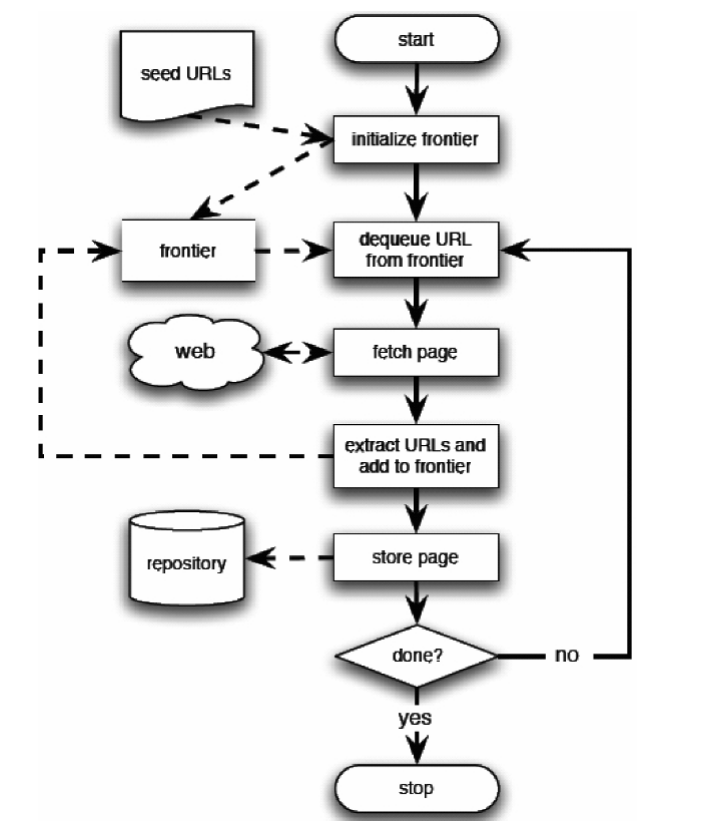
\includegraphics[width=.9\textwidth]{figures/basicCrawlAlgorithm.png}
    \caption{Diagram naivného algoritmu \label{o:basic_crawl_algorithm} \cite{dataMining}}
\end{figure}

\subsection{Fronta} \todo{Premenovat nadpis}
Fronta je centrálny prvok crawlera. Jej implementácia a nastavovanie odráža hlavné vlastnosti systému. 

Naivná implementácia požaduje FIFO dátovú štuktúru s deduplikovaním. Napríklad uchovanie navštívených adries. Pre malé, napríklad POC riešenia je to dostačujúce. 
Všeobecný crawler určený na široký web je typicky distribuovaný a potrebuje stránky znovu navštevovať pre zaručenie aktuálnosti zozbieraných informácii. Taktiež nemá dostatočné zdroje na pokrytie celej domény a musí selektovať adresy na navštívenie. Preto nepostačuje naivné riešenie, a fronta pre praktické využitie musí riešiť tieto požiadavky. 

\subsection{Politiky prehľadávania}
\textbf{Politika výberu} (selection policy) - určuje výber stránok podľa ich relevantnosti, popularite, aktuálnosti a kvalite. Taktiež pomocou nej vieme zúžiť prehľadávanú doménu, ak našim cieľom nie je celý web (napríklad iba e-shopy). Nikto nemá zdroje na prejdenie kaŽdej verejne dostupnej stránky, musí sa teda vybrať podmnožina s čo najrelevantnejšími informáciami. Preto je politika výberu kľúčová pre efektivitu crawlera. 

\textbf{Politika znovu navštívenia} (re-visit policy) - určuje ako často môže byť stránka znovu navštívená s cieľom získania aktuálnych informácii. Vo všeobecnosti platí, že čím vyššia frekvencia tým je menšia prehľadávaná podmnožina. 

\textbf{Politika zdvorilosti} (Politeness policy) - stránka si môže určiť, maximum a frekvenciu simultánnych requestov, taktiež sekciu stránok neprístupné pre botov. A to v súbore robots.txt \cite{robotsTxt}. 

\textbf{Politika paralelizácie} (Parallelization policy) - určuje, ako crawler rozdeľuje prácu a koordinuje súbežné prehľadávanie stránok. 

Politiky môžu byť statické - nastavenie pre jednotlivé stránky alebo skupiny stránok na základe ich domény. Napríklad zoznam stránok, ktorým dôverujeme a sú pre nás najpodstatnejšie. \todo{dobry nazov - napriklad index.sme.sk sme je domena})
Alebo dynamické - meniace sa podľa informácii získaných prehľadávaním. Napríklad analýzou obsahu stránky určíme relevantnosť stránok v tej istej doméne. 


\subsection{Vhodné vlastnosti všeobecného crawlera}

\textbf{Odolnosť} - voči pasciam proti botom alebo zle nadizajnovaným stránkam. Napríklad stránky generujúce nekonečnú množinu pod stránok, môžu zahltiť naivný crawler. 

\textbf{Škálovateľnosť} (scalability) - webový priestor sa rýchlo zväčšuje. Aby sa udržal podiel preskúmaných stránok, systém sa musí 
vedieť prispôsobiť. 

\textbf{Distribuovanosť} -  moderný web je mohutný a rýchlo sa meniaci. Pre získanie aktuálneho obrazu, potrebujeme obrovské množstvo dotazov za sekundu, čo vyžaduje distribuovaný systém. 

\textbf{Výkon a efektívnosť} - beh crawlera aj na obmedzenej doméne, vyžaduje robustný systém. Bez dôrazu na efektívnosť sa nám s obmedzenými prostriedkami nepodarí udržať požadovaný pomer spracovaných stránok z celej domény.

\textbf{Prioritizácia} - aplikovanie politiky výberu.

\textbf{Aktuálnosť} - aplikovanie politiky znovu navštívenia.

\textbf{Rozšíriteľnosť} - systém potrebuje spracovávať nové dátové formáty a protokoly. Architektúra by preto mala byť modulárna. 

\textbf{Etickosť} - systém by mal rešpektovať pravidlá v robots.txt.

\section{Použitie Web Crawlera}

\subsection{Použitie v priemysle}
Web Crawleri sú dôležitou súčasťou internetových vyhľadávačov, kde slúžia na zozbieranie korpusu webových stránok indexovaných vyhľadávačom. Pri čom nie je dôležitý iba obsah stránok ale aj vzťahy medzi nimi. Okrem toho sa používajú v mnohých ďalších aplikáciách, ktoré spracovávajú veľké množstvá webových stránok, ako sú ťažby dát z webov, porovnávacie nákupné enginy \footnote{ napríklad \url{https://www.heureka.sk/}} (comparison shopping engines). \cite{encykOfDatabases}.  

Taktiež na analýzu konkurencie pre dynamické určovanie ceny produktov. Napríklad úprava ceny na základe obsadenosti vstupných lístkov u resalarov (aero-linky). 
Môžu byť použité tiež na monitorovanie zmien a automatickú údržbu web-stránok. A to napríklad identifikovaním nefunkčných adries, kontrola generovanáho obsahu, nedosiahnuteľných assetov a monitorovanie výkonu stránky. \cite{crawlPageTesting}

\subsection{Použitie vo výskume}
Crawler je vhodným nástrojom na získavanie dát pre výskumné účely. Pomocou neho môžu vedci zbierať veľké množstvá dát. Tie môžu neskôr analyzovať a použiť na svoje výskumné účely. Crawler dokáže tieto dáta získať rýchlo a efektívne, čo umožňuje výskumníkom analyzovať trendy a vzory a vytvárať závery na základe veľkého množstva dát. Pre ilustráciu vymenujeme zopár praktických využití dát zozbieraných web crawlerom pre účely výskumu. 

\textbf{Analýza sociálnych sieti a médii} ako Instagram, Facebook, Twitter, Reddit, Youtube a pod. Obsahy príspevok, komentárov, reakcie užívateľov, dokonca aj multimédia ako fotky a videá sú zaujímavé dáta potrebné pre sledovanie nálad a trendov v spoločnosti. Na prípravu datasetov na tieto účely je vhodný crawler zameraný na konkrétne web stránky, v tomto prípade stránky sociálnych médii. Napríklad projekt SocialNetCrawler zbiera dáta na analýzu radikalizácie a extremizácie populácie \cite{socialNetCrawler}.

\textbf{Jazykovedné} skúmanie vývoja jazyka v 21. storočí vyŽaduje texty nie len z tlačených médii ale aj z online zdrojov. Crawler vie zozbierať texty a užitočné metadáta z verejných stránok v skúmanom jazyku a to filtrovaním podľa domény najvyššej úrovne (top level domain name) napríklad adresy končiace na .sk.

\textbf{Umelá inteligencia} potrebuje byť netrénovaná na obrovských datasetoch. Práve na ich prípravu sa môže pôužiť crawler. Napríklad zozbieranie otázok a odpovedí zo stránky Stack Overflow, za účelom vytrénovania AI chat bota. \cite{stackOverflowCrawl}

\subsection{Použitie v oblasti spravodajských webov}
Typickým príkladom sú textbf{portály zdieľajúce články} z rôznych spravodajských webov. Napríklad služba Google news\footnote{https://news.google.com/}. Táto a jej podobné služby prehľadávajú spravodajské weby a odporúčajú články používateľovi na základe jeho čitateľskej histórie a tém záujmu. Ak článok nie je kategorizovaný, využíva sa NLP (Natural language processing) na extrahovanie tém článkov (topic extraction/classification). Takto sa vedia obohatiť články o ďalšie informácie nevyskytujúce sa priamo na pozorovanej stránke.

\textbf{Agregácia správ v reálnom čase}, pri ktorej je potrebné za čo najkratší čas zozbierať a užívateľovi zobraziť informácie z vybranej skupiny stránok. Napríklad prehľad športových výsledkov. 

Crawlovanie sa taktiež používa pri \textbf{identifikácii nekvalitných článkov} - falošné správy a hoaxy \cite{fakeNews}. Okrem textov sa skúma aj zdrojovanie a prepojenia medzi stránkami. Toto použitie demonštruje dôležitosť získavania nie len obsahu stránok ale aj vzťahov medzi nimi, tie crawler dokáže spracovať do vhodnej formy pre analýzu. Napríklad do grafovej databázy. 



\section{POROVNANIE Existujúce crawlery pre naše použitie} \todo{asi premenovat}

Ako sme spomínali, cieľom je zozbieranie dát zo spravodajských webov na ich následné analyzovanie. To bude uskutočnené open-source nástrojmi Apache Spark a Apache OpenNLP. Tieto nástroje bežia na JVM (Java Virtual Machine). Uvedomujeme si, že máme malé zdroje na prevádzku. Preto potrebujeme open-source, ľahko udržiavané lightweight riešenie.

Scrapy 
Crawler4j
Apache Nutch 

